
\section{Trigonometry}

\subsection{The Basics}

Let $P$ be a point on a unit circle $x^2+y^2=1$. Let $\theta$ be the length
of the arc from $(1,0)$ to $P$, measured counterclockwise along the
circle. Then the coordinates of $P$ are
$(\cos\theta,\sin\theta)$.\footnote{The order is easy to remember-- it's
  alphabetical.}

\begin{figure}[htbp]
  \centering
  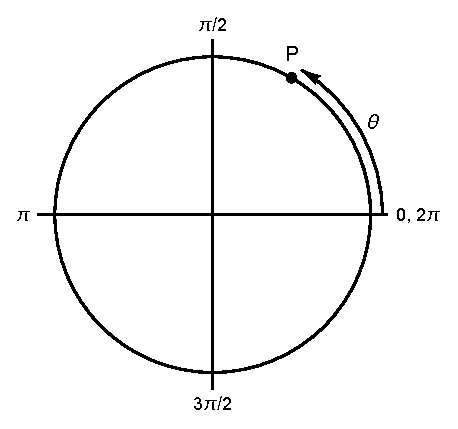
\includegraphics[width=0.5\textwidth]{trigtldr.eps}
\end{figure}

The measure of angles by the length of the arc is in units called
\textit{radians}. Recall the circumference of a circle is $C=2\pi r$,
and so the circumference of a unit circle is $2\pi$. Thus $\pi$ represents
a $180^\circ$ angle. Some common angles in radians are
$2\pi, \pi,\frac{\pi}{2}, \frac{\pi}{3}, \frac{\pi}{4}, \frac{\pi}{6}$, and
$\frac{3\pi}{2}$. To convert these to degrees simply replace $\pi$ with
$180$, and compute the fraction.

\vs

It should be self-evident that adding $2\pi$ to an angle results in the
angle itself; and that adding $\frac{\pi}{2}$ to an angle shifts it by
$90^{\circ}$. Further:
\[(\cos 0,\sin 0)=(1,0)\ \ \ \ \ \text{and}\ \ \ \ \ (\cos \frac{\pi}{2},\sin \frac{\pi}{2})=(0,1)\]

\clearpage
\subsection{Plotting}
It is not too difficult to plot trigonometric functions. Consider some
properties of cosine we've already seen (or can easily deduce):
$\cos 0=1$, $\cos \frac{\pi}{2}=0$, $\cos \pi=-1$. We've also seen that
$\cos{(x+2\pi)}=\cos x$. The $x$-axis below covers $[-3\pi, 3\pi]$ (i.e. a
total length of $6\pi$). Since cosine repeats every $2\pi$, we should
expect the graph to repeat thrice. And this is exactly what we see.
\begin{figure}[htbp]
  \centering
  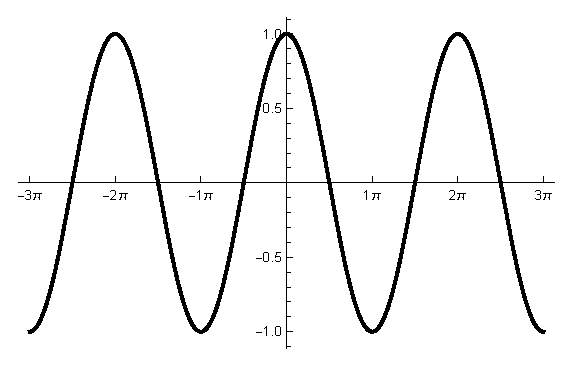
\includegraphics[width=.75\textwidth]{cosine.eps}
\end{figure}

We can easily increase the frequency by plotting $y=\cos cx$. Here we
double the frequency with $c=2$:
\begin{figure}[htbp]
  \centering
  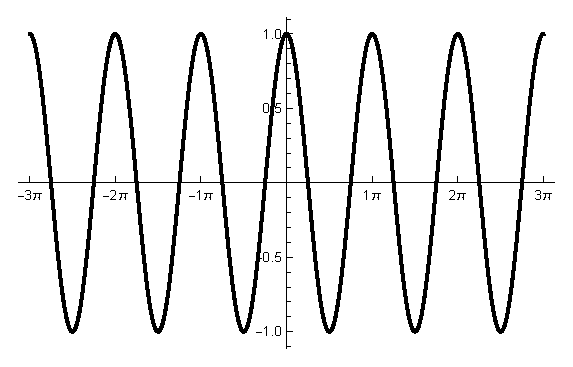
\includegraphics[width=.75\textwidth]{cosine2x.eps}
\end{figure}

%%% Local Variables:
%%% TeX-master: "precalc"
%%% End:
